\chapter{Introduction}
\lhead{\textit{Introduction}}
\rhead{\textit{METHODOLOGY}}

\lettrine[lines=2,slope=0pt,nindent=4pt]{\textbf{I}}{n} this chapter,
the three-stage methodology to build this report is developed as following:
1) inventory and sort of the \textsf{TrioCFD} database ; 2) development of a
new \texttt{PRM} template ; 3) running the \textsf{v1.8.3} of \textsf{TrioCFD} and description of \LaTeX~files.
In this first section we present a summary of those three stages before
giving accurate instructions and commands in next sections.

\section{Inventory and sort}
\lhead{\textit{Inventory and sort}}
\rhead{\textit{METHODOLOGY}}
Currently, the \texttt{TrioCFD} database contains 165 test
cases archived in different folders (see Table \ref{tab:List-of-folders}).
First, an important inventory work was carried out to sort the test
cases for targeting quickly the use of \texttt{TrioCFD} in different
CFD configurations. The inventory resulted in a single table with
plenty information (\texttt{LibreOffice} format), where the test cases
are classified into several subdomains of fluid flows. In this document,
some of them have been selected and detailed because 1) they are well-known
in the literature, 2) they present comparisons with other academic
or commercial CFD codes and 3) they present comparisons with experimental
data.

\begin{table}[H]
\begin{centering}
\begin{tabular}{ll}
\hline 
\textbf{Folders} & \textbf{Comments}\tabularnewline
\hline 
\texttt{\footnotesize{}/validation/share/Validation/Rapports\_automatiques/} & {\small{}files validating several }\texttt{\small{}baltik}\tabularnewline
\texttt{\footnotesize{}/Front\_tracking\_discontinu/share/Validation/Rapports\_automatiques/} & {\small{}sheets for }\texttt{\small{}baltik}{\small{} Front-tracking}\tabularnewline
\texttt{\footnotesize{}/P1NCP0RT/share/Validation/Rapports\_automatiques/} & \texttt{\small{}baltik}{\small{} P1NCP0RT}\tabularnewline
\texttt{\footnotesize{}/Rayonnement/share/Validation/Rapports\_automatiques/} & {\small{}radiation}\tabularnewline
\texttt{\footnotesize{}/LES/share/Validation/Rapports\_automatiques/} & {\small{}LES turbulence}\tabularnewline
\texttt{\footnotesize{}/Schema\_Euler\_Implicite\_Stationnaire/share/Validation/Rapports\_automatiques/} & {\small{}Steady state implicit Euler scheme}\tabularnewline
\texttt{\footnotesize{}/ALE/share/Validation/Rapports\_automatiques/} & {\small{}ALE method}\tabularnewline
\texttt{\footnotesize{}/Bas\_Reynolds/share/Validation/Rapports\_automatiques/} & {\small{}Low Reynolds turbulence models}\tabularnewline
\texttt{\footnotesize{}/Turbulence/share/Validation/Rapports\_automatiques/} & {\small{}Other turubulence models}\tabularnewline
\hline 
\end{tabular}
\par\end{centering}
\caption{\label{tab:List-of-folders}List of folders of \texttt{TrioCFD} test cases.}
\end{table}

Since version 1.9.0, the validation sheets are present in the Baltik necessary to execute them. Some of them can run only with TRUST (laminar and thermal laminar problems) but the choice was made to keep them in \texttt{TrioCFD}. All the validation sheets are accessible in the Baltik validation in the \texttt{/validation/share/Validation/Rapports\_automatiques/} directory.They are grouped here in accordance with the themes structuring this present validation report (Laminar Flow, Thermal Laminar Flow,...)
In addition, since version v1.9.0, the summary table of all these validation sheets is present in the appendix \textbf{Annexe A: List of TrioCFD \texttt{PRM} files} of this report.

%%%%%%%%%%%%%%%%%%%%%%%%%%%%%%%%%%%%%%%%%%%%%%%%%%%%%%%%%%%%%%%%%%%%%%%%%%%%%%
\section{Development of a new \textsf{PRM} template}
\lhead{\textit{Development of a new \textsf{PRM} template}}
\rhead{\textit{METHODOLOGY}}

For each datafile of test cases, the PDF file is generated by running
a bash script (command \texttt{Run\_fiche}) which acts on a \texttt{PRM}
file. A \texttt{PRM} file is a set of specific instructions for interfacing
the \LaTeX ~commands with the \texttt{TrioCFD} results post-processed
with \texttt{Gnuplot} or \texttt{Visit}. As its content differs following
the test cases, the generated PDF reports may be structured differently,
making them hard to read and to undersand. Consequently, a new \texttt{PRM} template
has been implemented in the present report to harmonize their content
for a more homogeneous rendering. Differences
between the old and new versions of the \texttt{PRM} template are detailed
in Section \ref{sec:New-PRM-syntax}. All validation sheets of this
report have been revised and enhanced by taking into account the new
\texttt{PRM} template.

%%%%%%%%%%%%%%%%%%%%%%%%%%%%%%%%%%%%%%%%%%%%%%%%%%%%%%%%%%%%%%%%%%%%%%%%%%%%%%
\section{Running with \textsf{v1.8.3} and \LaTeX~files}
\lhead{\textit{Running with \textsf{v1.8.3} and \LaTeX~files}}
\rhead{\textit{METHODOLOGY}}
For all test cases, the datafiles were run with the version \texttt{1.8.3}
of \texttt{TrioCFD} for checking the achievement of computations. The validation
database is launched on a new computer (PEGASI2). This is more efficient than
the previous one (is223288) since the validation database now runs in about 
3 days against more than 11 days with the previous one. 
The CPU time required to 1) compile \texttt{TRUST} and \texttt{TrioCFD}
and 2) run the 162 validation sheets.
The characteristics of the previous and new computer are given in Table \ref{tab:Computer-characteristics}.
For each validation sheet, the full documentation is automatically
generated via the \texttt{Run\_fiche} procedure. The validation
sheets associated with the daily elementary tests that run daily (not discussed
in more detail in this report) allow to obtain a coverage rate of
78.7\% of the keywords of \texttt{TrioCFD}. Finally, all selected sheets are
gathered in one single document. Precisions will be given on the \LaTeX~files
in Section \ref{chap:Validation-report-generation}.

\begin{table}[H]
\begin{centering}
\begin{tabular}{Sc Sc Sc}
\hline 
\textbf{COMPUTER} & \textbf{OPERATING SYSTEM} & \textbf{COMPILER} \tabularnewline
\hline 
\rowcolor{lightgray}\multicolumn{3}{Sc}{is223288@intra.cea.fr} \tabularnewline \hline
PC Linux Intel(R) Xeon(R) CPU E5-2620 0@2.00GHz & LINUX Fedora 26 & \textsf{GCC7.1.1}\tabularnewline
2 CPU - 6 physical cores per CPU & Kernel \textsf{gcc 7.1.1} & \textsf{MPICH3.2}\tabularnewline
\hline 
\rowcolor{lightgray}\multicolumn{3}{Sc}{pegasi2@intra.cea.fr} \tabularnewline \hline
PC Linux Intel(R) Xeon(R) Gold 5120 CPU @2.20GHz & CentOS 7.9.2009 & \textsf{GCC4.8.5}\tabularnewline
2 CPU - 14 physical cores per CPU & Kernel \textsf{gcc 4.8.5} & \textsf{MPICH3.2}\tabularnewline
\hline
\end{tabular}
\par\end{centering}
\caption{\label{tab:Computer-characteristics}Computer characteristics for
running the test cases database.}
\end{table}
%%%%%%%%%%%%%%%%%%%%%%%%%%%%%%%%%%%%%%%%%%%%%%%%%%%%%%%%%%%%%%%%%%%%%%%%%%%%%%%%%%%%%%%%
%%%%%%%%%%%%%%%%%%%%%%%%%%%%%%%%%%%%%%%%%%%%%%%%%%%%%%%%%%%%%%%%%%%%%%%%%%%%%%%%%%%%%%%%
\chapter{\label{chap:New-PRM-syntax}Overview of new \textsf{PRM} template}
\lhead{\textit{Overview of new \textsf{PRM} template}}
\rhead{\textit{METHODOLOGY}}
The \texttt{PRM} files are written in a specific template 
more user-friendly as described in the following.
The \texttt{PRM} sheet is then read by \texttt{Python} scripts which
convert it to \LaTeX~files.\smallskip\newline
For a better readability, an enhanced rendering and uniformity of
this document, a new \texttt{PRM} template has been implemented. This
new template provides a skeleton of the main items one should find in a CFD
study. By browsing it, the user will immediately know the system geometry,
the physical models, the boundary conditions, the numerical methods
and other unavoidable details. Each validation sheet included in this document
has been revised and improved with this new \texttt{PRM} template.
For some test cases, the physical content has been enriched with an extended
analysis and discussion. In subsection \ref{sec:Old-PRM-syntax},
we remind the structure of an old \texttt{PRM} syntax
(until version \textsf{v1.8.1}). The new syntax available since version \textsf{v1.8.2}
is then detail in subsection \ref{sec:New-PRM-syntax}.

%%%%%%%%%%%%%%%%%%%%%%%%%%%%%%%%%%%%%%%%%%%%%%%%%%%%%%%%%%%%%%%%%%%%%%%%%%%%%%%%%%%%%%%%
\section{\label{sec:Old-PRM-syntax}Old \texttt{PRM} syntax}
\lhead{\textit{Old-PRM-syntax}}
\rhead{\textit{METHODOLOGY}}
In the previous versions of \texttt{TrioCFD}, the formalism of a \texttt{PRM} was left to the hand of the writer of the file. 
The general structure was made up of a first part called \texttt{Parameters}. Then the writer could define as many chapters as he wanted via the keyword \textit{Chapter}.
The titles of the chapters were left to the discretion of the editor.
The methodology for writing the \texttt{PRM} as well as the keywords are explained in the \textcolor{blue}{\underline{PRM syntax}} section after launching \verb "trust -index".\newline \newline

In order to better understand the old structure, we will take the example of the \texttt{PRM} present in Chapter III.3 of
this report on a Cylinder in Laminar Cross Flow. The first keyword \textit{Parameters} was structured as follows:\newline
\begin{center}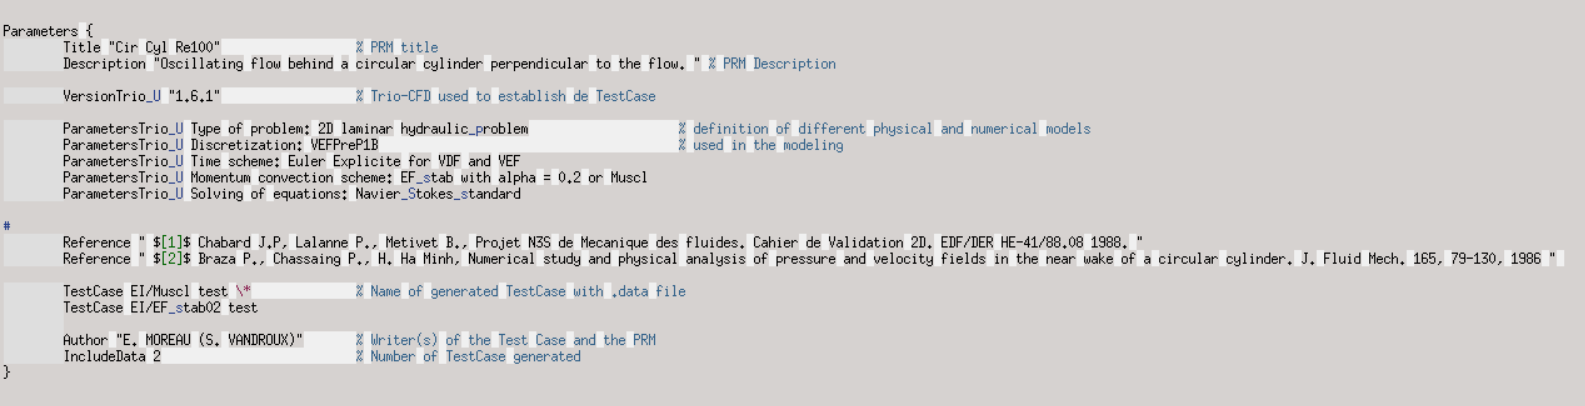
\includegraphics[width=16cm]{tools/parameters_PRM_1.png}\end{center}
\begin{center}\captionof{figure}{Original \texttt{PRM} syntax version - Parameters part}\end{center}

This part generates the first section of the \texttt{PRM} pdf entiteled \textit{1. Introduction} as follows:\newline
\setlength{\columnseprule}{0.5pt}
\begin{multicols}{2}
\begin{flushleft}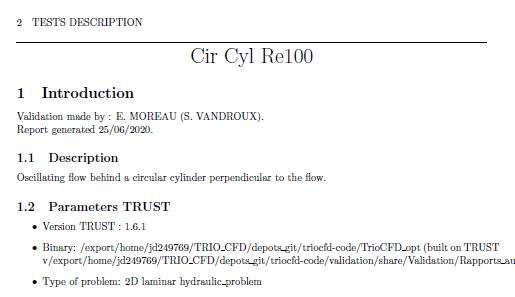
\includegraphics[width=8cm]{tools/parameters_PRM_1_pdf.png}\end{flushleft}
\columnbreak
\vspace{0.5cm}\begin{flushright}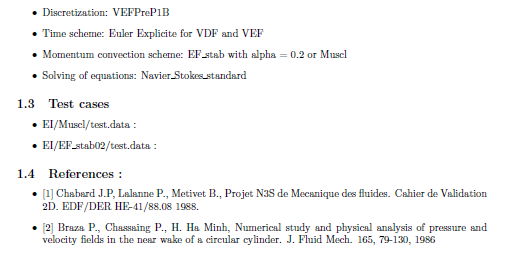
\includegraphics[width=8cm]{tools/parameters_PRM_2_pdf.png}\end{flushright}
\end{multicols}
\begin{center}\captionof{figure}{Original \texttt{PRM} syntax version - Generated introduction}\end{center}

After this first part, chapters can be freely added via the keword \verb"Chapter{ ... }" as follows:\newline
\begin{center}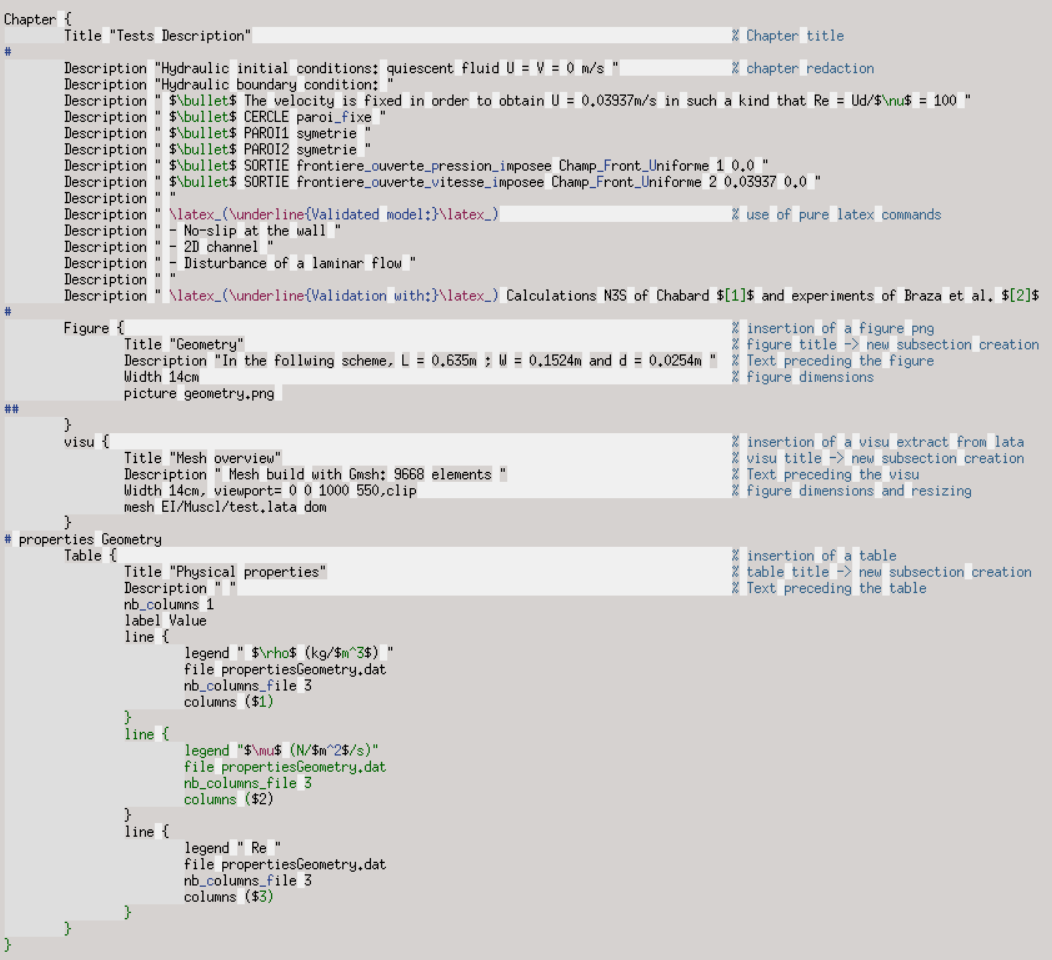
\includegraphics[width=12cm]{tools/chapter_PRM_1.png}\end{center}
\begin{center}\captionof{figure}{Original \texttt{PRM} syntax version - Chapter part}\end{center}

This part generates the second section of the \texttt{PRM} pdf entiteled \textit{2. Tests Description} as follows:\newline
\begin{center}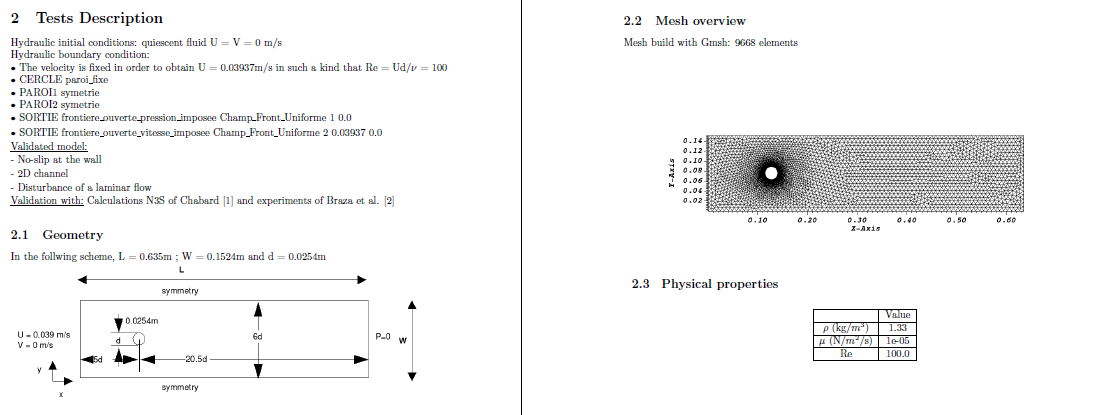
\includegraphics[width=15cm]{tools/chapter_PRM_1_pdf.png}\end{center}
\begin{center}\captionof{figure}{Original \texttt{PRM} syntax version - Generated chapter}\end{center}

%%%%%%%%%%%%%%%%%%%%%%%%%%%%%%%%%%%%%%%%%%%%%%%%%%%%%%%%%%%%%%%%%%%%%%%%%%%%%%%%%%%%%%%%
\section{\label{sec:New-PRM-syntax}New \textsf{PRM} syntax}
\lhead{\textit{New-PRM-syntax}}
\rhead{\textit{METHODOLOGY}}

\subsection{\label{subsec:General-improvements}General improvements}
Improvements have been made to the \texttt{Run\_fiche} procedure (managed
by \texttt{TRUST} code) and a new tag, \texttt{newvalidTrio}, has
been created to activate the new formalism. Some modifications have
been made in this new version for the generation of the \LaTeX~file from
the \texttt{PRM} file, without affecting the syntax of the \texttt{PRM}.
Thus, the \texttt{PRM} still includes the first block of instructions
entitled \texttt{Parameters} (see Section \ref{sec:Old-PRM-syntax})
which is followed by several blocks of instructions entitled by new
tags (or keywords). Those new keywords are listed in Section \ref{subsec:Modification-of-Python}.
The tag \texttt{Chapter} appearing in previous versions is removed and replaced
by many other tags. An additional improvement concerns the ``headers
and footers'' of PDF files. In earlier versions, the left header stated
the number and title of last section whereas the left footer stated
the test name. Now, the name is put on the left header, the left footer
is empty and the right footer still states the page number. That modification
was necessary for the concatenation of \LaTeX~files into one single
document and facilitates the readability.

\subsection{\label{subsec:Modification-of-Python}Modification of \texttt{Python}
script}
As seen in section \ref{sec:Old-PRM-syntax}, adding a new figure,
\texttt{visu}, or \texttt{table} automatically created
a new subsection. The title of that subsection is the same as the
figure name (respectively \texttt{visu} or \texttt{table}). Therefore,
too many irrelevant subsections were created and the title was used
as a caption for figures. In this work, the \texttt{Python} scripts
have been modified so that the title fields of figures (resp. \texttt{visu}
and \texttt{tables}) now correspond to the caption and their creation
no longer generates a subsection.\medskip\newline

\begin{table}[H]
\begin{centering}
	\begin{tabular}{lll}
	\hline 
	\noalign{\vskip0.3cm}
	\textbf{CONTENT OF NEW }\texttt{\textbf{\large{}PRM}}\textbf{ file} & $\qquad$ & \textbf{KEYWORDS OF NEW }\texttt{\textbf{\large{}PRM}}\textbf{ SYNTAX}\tabularnewline[0.2cm]
	\hline
	\noalign{\vskip0.1cm}
	\hline 
	\rowcolor{gray!10}%
	\begin{tabular}{c}
		\tabularnewline
		\textbf{1. Purpose}\tabularnewline
		\end{tabular} &  & %
	\begin{tabular}{lll}
		\textbf{English} &  & \textbf{French}\tabularnewline
		\texttt{\textbf{purpose~~~~~~~}} &  & \texttt{\textbf{objectif}}\tabularnewline
		\end{tabular}\tabularnewline
	\begin{tabular}{l}
		\textbf{2. Problem description}\tabularnewline
		{\small{}~~~~~2.1 Geometry}\tabularnewline
		{\small{}~~~~~2.2 Initial and boundary conditions}\tabularnewline
		{\small{}~~~~~2.3 Fluid properties}\tabularnewline
		{\small{}~~~~~2.4 Flow Physics}\tabularnewline
		\end{tabular} &  & %
	\begin{tabular}{lll}
		\texttt{\textbf{pb\_description}} &  & \tabularnewline
		\texttt{geometry} &  & \texttt{geometrie}\tabularnewline
		\texttt{\textbf{icbc}} &  & \texttt{\textbf{cicl}}\tabularnewline
		\texttt{\textbf{fluidprop}} &  & \texttt{\textbf{propfluide}}\tabularnewline
		\texttt{\textbf{flowphy}} &  & \texttt{\textbf{phyecou}}\tabularnewline
		\end{tabular}\tabularnewline
	\rowcolor{gray!10}%
	\begin{tabular}{l}
		\textbf{3. Case Setup}\tabularnewline
		{\small{}~~~~~3.1 Grid}\tabularnewline
		{\small{}~~~~~3.2 Model options}\tabularnewline
		{\small{}~~~~~3.3 Other options (calculations)}\tabularnewline
		\end{tabular} &  & %
	\begin{tabular}{lll}
		\texttt{\textbf{casesetup}} &  & \texttt{description\_cas}\tabularnewline
		\texttt{grid} &  & \texttt{maillage}\tabularnewline
		\texttt{model\_options~} &  & \texttt{options\_modele}\tabularnewline
		\texttt{other\_options} &  & \texttt{autres\_options}\tabularnewline
		\end{tabular}\tabularnewline
	\begin{tabular}{l}
		\textbf{4. Results}\tabularnewline
		{\small{}~~~~~3.1 Specific information}\tabularnewline
		{\small{}~~~~~3.2 Data plots}\tabularnewline
		\end{tabular} &  & %
	\begin{tabular}{lll}
		\texttt{\textbf{results~~~~~~~}} &  & \texttt{resultats}\tabularnewline
		none &  & \tabularnewline
		none &  & \tabularnewline
		\end{tabular}\tabularnewline
	\rowcolor{gray!10}%
	\begin{tabular}{c}
		\textbf{5. Conclusion}\tabularnewline
		\end{tabular} &  & %
	\begin{tabular}{l}
		\texttt{conclusion}\tabularnewline
	\end{tabular}\tabularnewline
	\begin{tabular}{c}
		\textbf{6. References}\tabularnewline
		\end{tabular} &  & %
	\begin{tabular}{l}
		\texttt{Reference} in block \texttt{\textbf{Parameters}}\tabularnewline
		\end{tabular}\tabularnewline
	\rowcolor{gray!10}%
	\begin{tabular}{c}
		\textbf{7. Datafile}\tabularnewline
		\end{tabular} &  & %
	\begin{tabular}{l}
		\texttt{TestCase} in block \texttt{\textbf{Parameters}} (if followed by \texttt{\textbf{\textbackslash{}{*}}})\tabularnewline
		\end{tabular}\tabularnewline
	\hline 
	\end{tabular}
\par\end{centering}
\end{table}
\begin{center}\captionof{table}{\label{tab:New-PRM-syntax:}New blocks of instructions in \texttt{PRM}
file: content (left) and corresponding keywords (right) in English or French.}.\end{center}

Moreover, the \texttt{PRM} is now interpreted line by line in order to allow better positioning
of the figures in the validation sheet. Previously, the \texttt{Description} fields were
all displayed together at the start of a section/subsection and the figures afterwards.
The \texttt{Python} script has been enhanced with the use of double dictionary to write, 
in the generated \LaTeX~file, the fields in the same order as that of the \texttt{PRM}.
It is therefore now possible to alternate the \texttt{Description}, \texttt{Figure},
\texttt{Visu} or \texttt{Table} fields and their order will be reproduced in the .tex file.\medskip\newline

In addition to these modifications, a new \texttt{PRM} syntax has
been implemented in order to present an identical content for all
validation sheets: now seven sections define all of them. Those sections
are listed in Table \ref{tab:New-PRM-syntax:} (left part). When writing
one \texttt{PRM} file, a new section corresponds to a new block of
instructions which must be declared by its corresponding keyword.
The list of keywords is presented in Table \ref{tab:New-PRM-syntax:}
(right part). All instructions inside the block must be enclosed by
braces: e.g \texttt{objectif \{...\}}, \texttt{pb\_description \{...\}},
\texttt{maillage \{...\}} and so on, where ``\texttt{...}'' means
several instructions on several lines.

Let us remind that in the old \texttt{PRM} syntax, the unique keyword
\texttt{Chapter} was defined as many times as necessary for defining
a new block of instructions. In particular, the number and name of
Sections were chosen by the authors (see Section \ref{sec:Old-PRM-syntax})
and the final rendering was different from one sheet to another.
With the new syntax, the blocks of instructions follow the first one
called \texttt{Parameters}. The second block of instructions is \texttt{objective
\{\}}, the third one is \texttt{pb\_description \{...\}}, and so on
until \texttt{conclusion \{...\}}. The block \texttt{Parameters} 
already existed in previous \texttt{PRM} version but minor modifications
have been brought. The commands are listed in Table \ref{tab:Required-keywords-in}
and an example of use is presented in Alg. \ref{alg:Example-of-use}.
The first one, \texttt{newvalidTrio}, is mandatory because this new
flag indicates the new \texttt{PRM} template. \texttt{TestCase} and
\texttt{ParametersTrio\_U} can be used multiple times in the block. 

\setlength{\tabcolsep}{0.1cm}
\renewcommand{\arraystretch}{1.25}
\begin{table}[H]
\begin{centering}
\begin{tabular}{lll}
\hline 
\textbf{Keywords} & $\qquad$ & \textbf{Use}\tabularnewline
\hline 
\texttt{newvalidTrio} &  & Required keyword to activate the new syntax\tabularnewline
\texttt{Title} &  & Defines title of the validation sheet\tabularnewline
\texttt{VersionTrio\_U} &  & First version of \texttt{TrioCFD} that performed validation\tabularnewline
\texttt{ParametersTrio\_U} &  & Comments that appear in Section 4.1 of the validation sheet\tabularnewline
\texttt{Reference} &  & References cited in the validation sheet\tabularnewline
\texttt{TestCase} &  & List of test cases run by \texttt{TrioCFD} and included in the validation
sheet\tabularnewline
\texttt{Author} &  & First authors who carried out this validation\tabularnewline
\texttt{IncludeData} &  & Command for including the entry datafile of TrioCFD\tabularnewline
\texttt{Description} &  & available in initial formalism, is no longer taken into account.\tabularnewline
\hline 
\end{tabular}
\par\end{centering}
\begin{center}\caption{\label{tab:Required-keywords-in}Keywords that can be used in block
\texttt{Parameters} for \texttt{PRM} files.}\end{center}
\end{table}

~
\begin{center}
\begin{algorithm}[H]
{\footnotesize{}\VerbatimInput{Exemple-Parameters-PRM.txt}}{\footnotesize\par}

\caption{\label{alg:Example-of-use}One example of block \texttt{Parameters}
(for brevity, few instructions are replaced by ``\texttt{...}'').}
\end{algorithm}\end{center}

The keyword \textbf{Description}, available in the inital formalism, is no longer taken into account.\smallskip\newline

In the old formalism, \texttt{Chapter} block was defined as many time as necessary with title chosen by the writer of the validation sheet (see Chapter II.1).
With this new formalism, predefined blocks can be used after the block \texttt{Parameters}.\smallskip\newline
\begin{description}
\item [{The~second~block}] is \texttt{Purpose} which can be activated
by the keyword \texttt{purpose} or \texttt{objectif}. In the PDF file,
the section \textbf{Purpose} is then created provided that the author
wants to fill it up. It explains which models will be validated in
the sheet and what sort of results (numerical, analytical, ...) \texttt{TrioCFD}
will be compared with.\smallskip\newline

\item [{The~third~block}] is \texttt{Problem description} which can be
activated by the keyword \texttt{pb\_description}. The section named
\textbf{Problem description} is then created. In this block, 4 sub-blocks
are available for creating 4 subsections which describe the geometry
of the physical domain defined to model the phenomenon, the initial
and boundary conditions used in the modeling, the fluid properties
and the flow physics. They can be activated with the following keywords:\smallskip\newline
\begin{table}[H]
\begin{centering}
\begin{tabular*}{16cm}{m{4.5cm} m{3cm} m{7.5cm}}
\hline 
\textbf{Keyword} & \textbf{Subsection number} & \textbf{Subsection title}\tabularnewline
\hline 
\textbf{geometry} or \textbf{geometrie} & 2.1 & Geometry\tabularnewline
\textbf{icbc} or \textbf{cicl} & 2.2 & Initial Conditions and Boundary Conditions\tabularnewline
\textbf{fluidprop} or \textbf{propfluide} & 2.3 & Fluid Properties\tabularnewline
\textbf{flowphy} or \textbf{phyecou} & 2.4 & Flow Physics\tabularnewline
\hline 
\end{tabular*}
\par\end{centering}
\caption{\label{tab:List-of-keyword-pbdes}List of keywords for the \texttt{Problem description} block.}
\end{table}

\item [{The~fourth~block}] entitled \texttt{Case Setup} block and activable
by the keyword casesetup or description\_cas has 3 available subsections
which can be defined by:\smallskip\newline
\begin{table}[H]
\begin{centering}
\begin{tabular*}{16cm}{m{4.5cm} m{3cm} m{7.5cm}}
\hline 
\textbf{Keyword} & \textbf{Subsection number} & \textbf{Subsection title}\tabularnewline
\hline 
\textbf{grid\_mesh} or \textbf{maillage} & 3.1 & Grid\tabularnewline
\begin{flushleft}\textbf{model\_options} or \textbf{options\_modele}\end{flushleft} & 3.2 & Model Options\tabularnewline
\begin{flushleft}\textbf{other\_options} or \textbf{autres\_options}\end{flushleft} & 3.3 & Other Options (calculation)\tabularnewline
\hline 
\end{tabular*}
\par\end{centering}
\caption{\label{tab:List-of-keyword-casesetup}List of keywords for the \texttt{Case Setup} block.}
\end{table}

\item [{The~fifth~block}] is an overview of the results of interest from
the validation sheet. This block entitled \textbf{Results} and activable
by the keyword \texttt{results} or \texttt{resultats} is composed
of two subsections. No keyword needed to activate those subsections
and the Results block definition is sufficient to create them.\\
The first, named \textbf{Validation Specific Informations} is automatically
generated and groups the fields \texttt{VersionTrio\_U} and \texttt{ParametersTrio\_U}
defined in the \texttt{Parameters} block. The performance table for
each test case is automatically inserted at the end of this subsection.\\
The second subsection, entitled \textbf{Plot Data} is generated by
reading line by line the keywords \texttt{Description}, \texttt{Figure},
\texttt{Visu} or \texttt{Table} defined by the author in the block.
Respecting this order allows an easier writing and reading of the \texttt{PRM}
file.

\item [{The~last~block}] named \texttt{Conclusion} defined by the keyword
\texttt{conclusion} has no subsection and is filled by line-by-line
reading of the \texttt{PRM} like the other blocks. Here is an assessment
of the validation status of the sheet.

\item [{The~two~last~sections}] of the validation sheet, \textbf{References}
and \textbf{Data Files}, are automatically generated respectively
from keywords \texttt{Reference} and \texttt{TestCase} inside the
\texttt{Parameters} block.\medskip\newline
\end{description}
Four instructions can be used inside all blocks and sub-blocks: \texttt{Description},
\texttt{Figure}, \texttt{Visu} and \texttt{Table} that can be repeated
as many times as necessary and in the desired writing order.

%%%%%%%%%%%%%%%%%%%%%%%%%%%%%%%%%%%%%%%%%%%%%%%%%%%%%%%%%%%%%%%%%%%%%%%%%%%%%%%%%%%%%%%%
%%%%%%%%%%%%%%%%%%%%%%%%%%%%%%%%%%%%%%%%%%%%%%%%%%%%%%%%%%%%%%%%%%%%%%%%%%%%%%%%%%%%%%%%
\chapter{\label{chap:Validation-report-generation}\LaTeX~files and report generation}
\lhead{\textit{\LaTeX~files and report generation}}
\rhead{\textit{METHODOLOGY}}
The procedure for generating this report is flexible and automated.
As a matter of fact, each author can work independently on each validation
sheet with the new \texttt{PRM} template (Section \ref{sec:New-PRM-syntax}).
Moreover, all parts of this document are written in several \LaTeX~files
with clear names (Section \ref{sec:LaTeX_files}). A new one can
easily be added. Finally a shell script automates the following tasks:
gathering all \LaTeX~files, cleaning all sheets texfiles (Section
\ref{sec:Generating-the-report}) and making one single PDF document.
%%%%%%%%%%%%%%%%%%%%%%%%%%%%%%%%%%%%%%%%%%%%%%%%%%%%%%%%%%%%%%%%%%%%%%%%%%%%%%%%%%%%%%%%
\section{\label{sec:LaTeX_files}\LaTeX~files}
\lhead{\textit{\LaTeX~files}}
\rhead{\textit{METHODOLOGY}}
The main \LaTeX~file of this report is named \texttt{validation\_report\_TrioCFD.tex}.
The file contains the standard instructions \texttt{\textbackslash{}documentclass},
\texttt{\textbackslash{}usepackage},\texttt{ \textbackslash{}begin\{document\}}
and \texttt{\textbackslash{}end\{document\}}. The eight parts of this
report are written in eight separated \LaTeX~files (see their names
in Tab. \ref{tab:LaTeX_files}). Those files are included in the main
with the command \texttt{\textbackslash{}input\{\}} (e.g. \texttt{\textbackslash{}input\{./part1-introduction.tex\}}).

\begin{table}[H]
\begin{centering}
\begin{tabular}{ll}
\hline 
\textbf{\LaTeX~file} & \textbf{Comment}\tabularnewline
\hline 
\texttt{validation\_report\_TrioCFD.tex} & Main file\tabularnewline
\texttt{part1-introduction.tex} & File included\tabularnewline
\texttt{part2-methodology.tex} & id\tabularnewline
\texttt{part3-laminar.tex} & id\tabularnewline
\texttt{part4-thermallaminar.tex} & id\tabularnewline
\texttt{part5-turbulent.tex} & id\tabularnewline
\texttt{part6-thermalturbulent.tex} & id\tabularnewline
\texttt{part7-FT.tex} & id\tabularnewline
\texttt{part8-conclusion.tex} & id\tabularnewline
\hline 
\end{tabular}
\par\end{centering}
\caption{\label{tab:LaTeX_files}\LaTeX~files of this report.}
\end{table}

The validation sheets are also included in the main by the same command.
All of them are placed inside the folder \texttt{./fiches} containing
subfolders of all test cases e.g.\texttt{ Poiseuille\_flow\_2D\_VDF\_VEF},\texttt{
Cir\_Cyl\_Re100}, \texttt{OBI\_diffuser\_VEF\_k\_eps}, and so on ...
Inside them, the \LaTeX~file of each validation sheet is called
\texttt{fic.tex} which can be found in the directory \texttt{./build/.tmp/}.
For instance, instruction for including the validation sheet of ``Lid
driven cavity flow'' is:\newline
\texttt{ \textbackslash{}input\{./fiches/Lid\_driven\_cavity/build/.tmp/fic.tex\}}.
All these \texttt{fic.tex} files were generated by \texttt{Python} scripts reading
the \texttt{PRM} template.
%%%%%%%%%%%%%%%%%%%%%%%%%%%%%%%%%%%%%%%%%%%%%%%%%%%%%%%%%%%%%%%%%%%%%%%%%%%%%%%%%%%%%%%%
\section{\label{sec:Generating-the-report}New shell script for gathering all \texttt{.tex} files}
\lhead{\textit{New shell script for gathering all \texttt{.tex} files}}
\rhead{\textit{METHODOLOGY}}
The folder \texttt{fiches} and all subfolders of test cases are created
by \texttt{generer\_rapport\_valid.unix}. For all test cases, the
first task of this shell script is to copy the \texttt{build} directory
of \texttt{TrioCFD} results in corresponding subfolders. The second
task is to clean each \texttt{fic.tex} file in order to be included
in the main \LaTeX~file. Finally the instruction \texttt{pdflatex
validation\_report\_TrioCFD.tex} compiles and generates the PDF file.

%%%%%%%%%%%%%%%%%%%%%%%%%%%%%%%%%%%%%%%%%%%%%%%%%%%%%%%%%%%%%%%%%%%%%%%%%%%%%%%%%%%%%%%%
\section{Enhancement}
\lhead{\textit{Enhancement}}
\rhead{\textit{METHODOLOGY}}
For future versions of this document, the shell script will be enhanced.
Currently, adding a new sheet to the report is carried out manually
in the shell script. It would be more comfortable to automate the
procedure by copying all \texttt{PRM} files which contains the keyword
\texttt{newvalidTrio}, copy the build directory and do a loop inside
the shell script.
